\documentclass[a4paper,twoside,12pt]{article}  
\usepackage{amsmath}					% balicek pro matiku
\usepackage{color}
\usepackage{footnote}					% poznámka pod čarou
\usepackage{url}						% url odkazy
\DeclareUrlCommand\url{\def\UrlLeft{<}\def\UrlRight{>} \urlstyle{tt}}
\usepackage{float}						% plovoucí prostředí
\usepackage[utf8]{inputenc}			% kódování	
\usepackage[czech]{babel}				% čeština
% \usepackage{icomma}      				% není mezera za desetinnou čárkou
\usepackage{enumerate}      			% seznamy 
\usepackage{amsfonts}      				% množiny Z,R,N dvojitě
\usepackage{amssymb}      				% znaky úhlu a tak

\usepackage[pdftex]{graphicx}
\usepackage{setspace}
\usepackage{multicol}					% tabulka, slučování sloupců
\usepackage{multirow}					% tabulka, slučování řádků
\usepackage{fancyhdr}					% záhlaví a zápatí stránky
\usepackage{hyperref}					% reference pro \tableofcontents
	
\DeclareGraphicsExtensions{.pdf,.png,.jpg}	% nahrávání obrázků, rošíření
\newcommand{\degree}[1][]{\ensuremath{{#1}^\circ}} 

\usepackage[a4paper, top=2cm, left=2.5cm, right=2.5cm, includefoot]{geometry}		% nastavení okrajů
\newcommand{\at}{\makeatletter @\makeatother}


\usepackage[]{algorithm2e}				% balíček pro pseudokód

\graphicspath{{obrazky/}} 				% umístění obrázků
\usepackage[numbers]{natbib}
\usepackage{notoccite}
		
\clubpenalty 10000		% penalizace sirotků, sirotek: poslední řádek odstavce je na nové stránce
\widowpenalty 10000		% penalizace vdov, vdova: první řádek nového odstavce je na konci stránky

\usepackage{chngcntr} 
\counterwithin{figure}{section} 
\counterwithin{table}{section} 

\renewcommand{\baselinestretch}{1.5}	% řádkování 1,5

\begin{document}
	\pagestyle{empty}
	
	\title{Semestrální práce}
	\author{Karavaev Aleksei}
	\date{\today}
 
	\begin{titlepage}
 		\begin{center}
 		\textsc{\large{České vysoké učení technické v Praze}}\\
 		\textsc{\large{Fakulta biomedicínského inženýrství}}\\
		\large{Katedra biomedicínské informatiky}\\[2cm]
		
		\begin{figure}[!h]
			\centering
 			
\includegraphics[width=0.3\textwidth]{symbol_cvut_konturova_verze}
 		\end{figure}
 		
		\Large{EEG}\\
		\Large{Úkol 3} 
		\vfill
		\end{center}		
		Autor práci: \hspace{0.55cm} Karavaev Aleksei\\
				
		\begin{center}
		květen 2020
		\end{center}
		\clearpage


	\end{titlepage}

	\pagestyle{fancy}	%cislovani stranek zacina odsud  	% Předem definované záhlaví a zápatí.
\section{Připrava signálu}
Na začátku jsem vyfiltroval každý ze souboru pomoci pásmové zadrže 0,5-30 Hz. Tento filtr by měl zachovat užitečné frekvenci EEG signálu.  Zkoušel jsem odfiltrovat i blikání, ale nezlepšilo to kvalitu výsledku. Na signál jsem aplikoval fourerovou transformaci pro získaní amplitudové frekvenční charakteristiky signálu. Tuto charakteristiku jsem dal zpracovával.
\section{Klasifikace}
Pro klasifikaci jsem použil konvoluční neuronovou sít. Měla by sama vytěžit příznaky z amplitudové frekvenční charakteristiky signálu. 
\begin{figure}[H]
\begin{center}
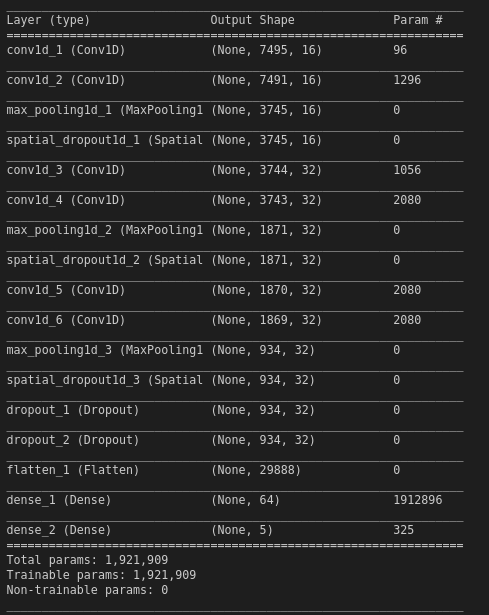
\includegraphics[width=0.6\textwidth]{neuronka}
\caption{Struktura neuronové sitě}
\label{img:neuronka}
\end{center}
\end{figure}
\section{Přesnost klasifikaci na testovacích datech}
Pro každý signál jsem přeučil algoritmus. Na trénovacích datech pro signály 1 a 5 dosahoval přesnosti až 75\%. U signálů 2,3,4 přesnost byla značně menší(30-40\%). Což mohlo být způsobený špatnou kvalitou dat. Zkoušel jsem tunit sít, ale nepřineslo to značného zlepšení kvality výsledků.Nevyvažoval jsem přiznáky, což taky mohlo být příčinou špatného výstupu.

\clearpage
		\addcontentsline{toc}{section}{Seznam obrázků}
		\listoffigures 		% seznam obrázků
		\clearpage
	
	\setlength{\parskip}{0.5cm}		%mezera za odstavci
		
	
\end{document}
	
	